\documentclass[submit]{../harvardml}

\course{CS1810-S25}
\assignment{Assignment \#6}
\duedate{11:59PM EST, May 2 2025}
\newcommand{\attr}[1]{\textsf{#1}}
\usepackage[OT1]{fontenc}
\usepackage{float}
\usepackage[colorlinks,citecolor=blue,urlcolor=blue]{hyperref}
\usepackage[pdftex]{graphicx}
\usepackage{../common} 
\usepackage{fullpage}
\usepackage{amsmath}
\usepackage{amssymb}
\usepackage{color}
\usepackage{todonotes}
\usepackage{listings}
\usepackage{bm}
\usepackage{enumitem}
\usepackage{tikz}
\usepackage{xifthen}
\usepackage{soul}
\usepackage{framed}
<<<<<<< HEAD
\usepackage{graphicx}
\usepackage{subfig}        % provides \subfloat
\usepackage{listings} % Code listings

\lstset{
  language=Python,
  basicstyle=\small\ttfamily,
  frame=single,
  backgroundcolor=\color{white},
  breaklines=true,
  showstringspaces=false
}
=======

>>>>>>> 029a483aa01e3c3745c42e8094d4dbc952e22f1f

\usepackage[mmddyyyy,hhmmss]{datetime}

\definecolor{verbgray}{gray}{0.9}

\lstnewenvironment{csv}{
  \lstset{backgroundcolor=\color{verbgray},
  frame=single,
  framerule=0pt,
  basicstyle=\ttfamily,
  columns=fullflexible}}{}

\newcommand{\mueps}{\mu_{\epsilon}}
\newcommand{\sigeps}{\sigma_{\epsilon}}
\newcommand{\mugam}{\mu_{\gamma}}
\newcommand{\siggam}{\sigma_{\gamma}}
\newcommand{\muzp}{\mu_{p}}
\newcommand{\sigzp}{\sigma_{p}}
\newcommand{\gauss}[3]{\frac{1}{2\pi#3}e^{-\frac{(#1-#2)^2}{2#3}}}

%%%%%%%%%%%%%%%%%%%%%%%%%%%%%%%%%%
%% Solution environment
\newenvironment{solution}
  {\color{blue}\section*{Solution}}
{}
% \excludecomment{solution} % UNCOMMENT TO HIDE SOLUTIONS
%%%%%%%%%%%%%%%%%%%%%%%%%%%%%%%%%%

\begin{document}
\begin{center}
{\Large Homework 6: Inference in Graphical Models, MDPs}\\
\end{center}

\subsection*{Introduction}

In this assignment, you will practice inference in graphical models as
well as MDPs/RL.

\subsection*{Resources and Submission Instructions}

For readings, we recommend \href{http://incompleteideas.net/book/the-book-2nd.html}{Sutton and Barto 2018, Reinforcement Learning: An Introduction}, \href{https://harvard-ml-courses.github.io/cs181-web/}{CS181  Lecture Notes}, and Section 10 and 11 Notes.

Please type your solutions after the corresponding problems using this \LaTeX\ template, and start each problem on a new page.

Please submit the writeup PDF to the Gradescope assignment `HW6'. Remember to assign pages for each question.  \textbf{You must include any plots in your writeup PDF.} Please submit your \LaTeX file and code files to the Gradescope assignment `HW6 - Supplemental.' The supplemental files will only be checked in special cases, e.g. honor code issues, etc. Your files should be named in the same way as we provide them in the repository, e.g. \texttt{hw0.pdf}, etc.
\\

\newpage

\begin{problem}[Hidden Markov Models, 15 pts]
In this problem, you will be working with one-dimensional Kalman filters, which are \textit{continuous-state} Hidden Markov Models. Let $z_0, z_1, \cdots , z_t$ be the hidden states of the system and $x_0, x_1, \cdots, x_t$ be the observations produced. Then, state transitions and emissions of observations work as follows:
  \begin{eqnarray*}
    z_{t+1} &= z_{t} + \epsilon_{t} \\
    x_{t} & = z_{t} + \gamma_{t}
  \end{eqnarray*}
 where $\epsilon_t \sim N(0,\sigeps^2)$ and $\gamma_t \sim N(0,\siggam^2)$. The value of the first hidden state follows the distribution $z_0 \sim N(\muzp,\sigzp^2)$.

\begin{enumerate}
  \item Draw the graphical model corresponding to the one-dimensional Kalman filter.
  \item In this part we will walk through the derivation of the conditional distribution of $z_t|(x_0, \cdots, x_{t})$.
  \begin{enumerate}
      \item How does the quantity $p(z_t| x_0, \cdots, x_{t})$ relate to $\alpha_t(z_t)$ and $\beta_t(z_t)$ from the forward-backward algorithm for HMMs?  What is the operation we are performing called?
      \item The above quantity $p(z_t|x_0, \cdots, x_t)$ is the PDF for a Normal distribution with mean $\mu_t$ and variance $\sigma_t^2$. We start our derivation of $\mu_t$ and $\sigma_t^2$ by writing:
      \begin{align*}
          p(z_t|x_0, \cdots, x_t) \propto p(x_t|z_t)p(z_t|x_0, \cdots x_{t-1})
      \end{align*}
      What is $p(x_t|z_t)$ equal to?
      \item Suppose we are given the mean and variance of the distribution $z_{t-1}|(x_0, \cdots, x_{t-1})$ as $\mu_{t-1}$, $\sigma^2_{t-1}$. What is $p(z_t|x_0, \cdots x_{t-1})$ equal to? 
      
      \textbf{Hint 1}: Start by marginalizing out over $z_{t-1}$.
      
      \textbf{Hint 2}: You may cite the fact that 
      \[\int N(y-x ; \mu_a, \sigma^2_a)N(x ; \mu_b, \sigma^2_b)dx = N(y ; (\mu_a + \mu_b), (\sigma^2_a + \sigma^2_b))\]
      \item Combine your answers from parts (b) and (c) to get a final expression for $p(z_t|x_0, \cdots, x_t)$. Report the mean $\mu_t$ and variance $\sigma_t^2$ of this Normal.

      \textbf{Hint 1}: Rewrite $N(x_t; z_t, \siggam^2)$ as $N(z_t; x_t, \siggam^2)$.
      
      \textbf{Hint 2}: You may cite the fact that 
      \[N(x; \mu_a, \sigma^2_a)N(x; \mu_b, \sigma^2_b) \propto N\left(x; \frac{\sigma^2_b}{\sigma^2_a+\sigma^2_b}\mu_a + \frac{\sigma^2_a}{\sigma^2_a+\sigma^2_b}\mu_b, \ \left(\frac{1}{\sigma^2_a} + \frac{1}{\sigma^2_b}\right)^{-1}\right)\]
  \end{enumerate}
  \item Interpret $\mu_t$ in terms of how it combines observations from the past with the current observation. 
\end{enumerate}
\end{problem}


\newpage

\begin{solution}
<<<<<<< HEAD
    \begin{enumerate}
        \item The graphical model is 
        \begin{figure}[H]
            \centering
            \includegraphics[width=0.6\linewidth]{hw6/img_output/1a.pdf}
        \end{figure}

        \item 
            \begin{enumerate}
                \item We have
                $$p(z_t| x_0,\dots,x_t)\propto p(x_0,\dots,x_t, z_t) =  \alpha_t(z_t)\,\beta_t(z_t)$$
                Therefore we multiply the forward message $\alpha_t$ by the backward message $\beta_t$ and renormalize. This operation is called smoothing.

                \item Recall that $\gamma_t \sim N(0, \siggam^2)$ and $x_t = z_t + \gamma_t$. Therefore, conditioning on $z_t$, $z_t$ is a constant and becomes a location shift by Normal properties
                $$x_t | z_t = z_t + \gamma_t \sim N(z_t, \sigma^2_\gamma)$$
                Therefore, using the Normal PDF
                $$p(x_t| z_t) = N(x_t; z_t, \siggam^2) = \frac{1}{\siggam\sqrt{2\pi}} \exp\Bigl(-\frac{1}{2\siggam^2 (x_t - z_t)^2}\Bigr)$$

                \item Per the hint, we start by marginalizing out $z_{t-1}$
                $$p(z_t| x_0,\dots,x_{t-1}) =\int p(z_t| z_{t-1})\,p(z_{t-1}| x_0,\dots,x_{t-1})dz_{t-1}$$
                To find the distribution of $z_t | z_{t-1}$, recall that we are given $z_t = z_{t-1} + \epsilon_{t-1}$ with $\epsilon_{t-1} \sim N(0,\sigeps^2)$. Therefore, by similar logic from part 2(b), we know that conditioning on $z_{t-1}$ is equivalent to a location shift and thus
                $$p(z_t | z_{t-1}) = N(z_t; z_{t-1}, \sigeps^2) = N(z_t - z_{t-1}; 0, \sigeps^2)$$
                Then, by Normal-Normal conjugacy, we know that the $z_{t-1}| x_{0},\dots, x_{t-1}$ is Normal. Since we are given that the distribution has mean $\mu_{t-1}$ and variance $\sigma_{t-1}^2$, then $p(z_{t-1}| x_{0},\dots, x_{t-1})= N(z_{t-1}; \mu_{t-1},\sigma_{t-1}^2)$. Therefore, citing the fact in hint 2, we have
                $$ p(z_t| x_0,\dots,x_{t-1}) =  \int N(z_t - z_{t-1}; 0, \sigeps^2) N(z_{t-1}; \mu_{t-1},\sigma_{t-1}^2)dz_{t-1} = N(z_{t}; \mu_{t-1},\sigma_{t-1}^2+\sigma_\epsilon^2)$$

                \item By Bayes rule we have
                $$p(z_t| x_0,\dots,x_t) = \frac{p(x_t|z_t,x_0,\dots,x_{t-1})p(z_t|x_0,\dots,x_{t-1})}{p(x_t|x_0,\dots,x_{t-1})} \propto p(x_t|z_t,x_0,\dots,x_{t-1})p(z_t|x_0,\dots,x_{t-1})$$
                However, by the HMM assumption that at step $t$ the observed emission $x_t$ only depends on the current state $z_t$, we have
                $$p(x_t|z_t,x_0,\dots,x_{t-1}) = p(x_t|z_t)$$
                Recall from part (b) that $p(x_t |z_t) = N(x_t; z_t, \siggam^2) = N(z_t; x_t, \siggam^2)$, where we rewrote according to Hint 1. In addition, recall from part (c) that $p(z_t| x_0,\dots,x_{t-1}) = N(z_{t}; \mu_{t-1},\sigma_{t-1}^2+\sigma_\epsilon^2)$. Therefore, by Hint 2
                $$p(z_t| x_0,\dots,x_t)\propto N(z_t;x_t,\siggam^2)\;N(z_t;\mu_{t-1},\sigma_{t-1}^2+\sigeps^2) \propto N(z_t; \mu_t, \sigma_t^2)$$
                Where the mean $\mu_t$ is
                $$\mu_t = \frac{x_t(\sigma_{t-1}^2+\sigeps^2) + \mu_{t-1}\siggam^2}{\sigma_{t-1}^2+\sigeps^2 + \siggam^2}$$
                $$\sigma_t^2 =\Bigl(\frac{1}{\siggam^2} + \frac{1}{\sigma_{t-1}^2+\sigeps^2}\Bigr)^{-1}$$
            \end{enumerate}

        \item The posterior mean $\mu_t$ is a weighted average of the prediction $\mu_{t-1}$ and the new observation $x_t$, with weights given by their precisions (in the form of variance). Therefore it balances past information with the current measurement according to their uncertainties.
    \end{enumerate}
=======
	Your solution here.
>>>>>>> 029a483aa01e3c3745c42e8094d4dbc952e22f1f
\end{solution}

\newpage

\begin{problem}[Policy and Value Iteration, 15 pts]

You have a robot that you wish to collect two parts in an environment
and bring them to a goal location.  There are also parts of the
environment that you wish the robot avoid to reduce wear on the floor.

Eventually, you settle on the following way to model the environment
as a Gridworld.  The ``states'' in Gridworld are represented by
locations in a two-dimensional space.  Here we show each state and its
reward:

\begin{center}
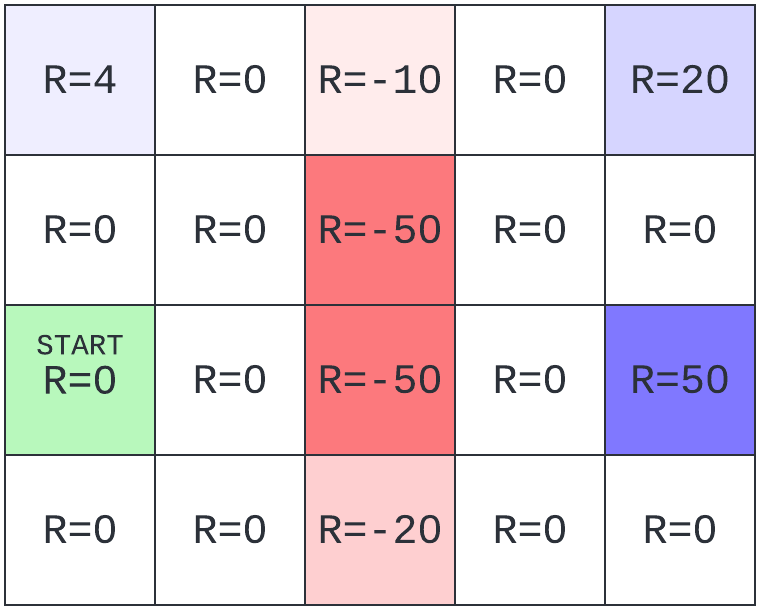
\includegraphics[width=3in]{img_input/gridworld.png}
\end{center}

The set of actions is \{N, S, E, W\}, which corresponds to moving north (up), south (down), east (right), and west (left) on the grid. Taking an action in Gridworld does not always succeed with probability
$1$; instead the agent has probability $0.1$ of ``slipping'' into a
state on either side, but not backwards.  For example, if the agent tries to move right from START, it succeeds with probability 0.8, but the agent may end up moving up or down with probability 0.1 each. Also, the agent cannot move off the edge of the grid, so moving left from START will keep the agent in the same state with probability 0.8, but also may slip up or down with probability 0.1 each. Lastly, the agent has no chance of slipping off the grid - so moving up from START results in a 0.9 chance of success with a 0.1 chance of moving right.

Also, the agent does not receive the reward of a state immediately upon entry, but instead only after it takes an action at that state. For example, if the agent moves right four times (deterministically, with no chance of slipping) the rewards would be +0, +0, -50, +0, and the agent would reside in the +50 state. Regardless of what action the agent takes here, the next reward would be +50.

In this problem, you will first implement policy and value iteration in this setting and discuss the policies that you find.  Next, you will interrogate whether this approach to modeling the original problem was appropriate.

\end{problem}
\newpage

\begin{framed}
\textbf{Problem 2} (cont.)\\

Your job is to implement the following three methods in file \texttt{homework6.ipynb}. Please use the provided helper functions \texttt{get\_reward} and \texttt{get\_transition\_prob} to implement your solution. \emph{Do not use any outside code.  (You may still collaborate with others according to the standard collaboration policy in the syllabus.)}  

\textbf{Important: } The state space is represented using integers, which range from 0 (the top left) to 19 (the bottom right). Therefore both the policy \texttt{pi} and the value function \texttt{V} are 1-dimensional arrays of length \texttt{num\_states = 20}. Your policy and value iteration methods should only implement one update step of the iteration - they will be repeatedly called by the provided \texttt{learn\_strategy} method to learn and display the optimal policy. You can change the number of iterations that your code is run and displayed by changing the $\texttt{max\_iter}$ and $\texttt{print\_every}$ parameters of the $\texttt{learn\_strategy}$ function calls at the end of the code.

Note that we are doing infinite-horizon planning to maximize the expected reward of the traveling agent. For parts 1-3, set discount factor $\gamma = 0.7$.

\begin{itemize}
    \item[1a.]  Implement function \texttt{policy\_evaluation}.  Your
      solution should learn value function $V$, either using a closed-form expression or iteratively using
      convergence tolerance $\texttt{theta = 0.0001}$ (i.e., if
      $V^{(t)}$ represents $V$ on the $t$-th iteration of your policy
      evaluation procedure, then if $|V^{(t + 1)}[s] - V^{(t)}[s]|
      \leq \theta$ for all $s$, then terminate and return $V^{(t + 1)}$.)

    \item[1b.] Implement function \texttt{update\_policy\_iteration} to update the policy \texttt{pi} given a value function \texttt{V} using \textbf{one step} of policy iteration.
    
    \item[1c.] Set \texttt{max\_iter = 4}, \texttt{print\_every = 1} to show the learned value function and the associated policy for the first 4 policy iterations. Do not modify the plotting code. Please fit all 4 plots onto one page of your writeup.
    
    \item [1d.] Set \texttt{ct = 0.01} and increase \texttt{max\_iter} such that the algorithm converges. Include a plot of the final learned value function and policy. How many iterations does it take to converge? Now try \texttt{ct = 0.001} and \texttt{ct = 0.0001}. How does this affect the number of iterations until convergence?
      
    \item [2a.] Implement function
      \texttt{update\_value\_iteration}, which performs \textbf{one step} of value iteration to update \texttt{V}, \texttt{pi}.
      
    \item [2b.] Set \texttt{max\_iter = 4}, \texttt{print\_every = 1} to show the learned value function and the associated policy for the first 4 value iterations. Do not modify the plotting code. Please fit all 4 plots onto one page of your writeup.
    
    \item [2c.] Set \texttt{ct = 0.01} and increase \texttt{max\_iter} such that the algorithm converges. Include a plot of the final learned value function and policy. How many iterations does it take to converge? Now try \texttt{ct = 0.001} and \texttt{ct = 0.0001}. How does this affect the number of iterations until convergence?
    
    \item[3.] Compare and contrast the number of iterations, time per iteration, and overall runtime between policy iteration and value iteration. What do you notice?
    
    \item[4.] Plot the learned policy with each of $\gamma \in (0.6,0.7,0.8,0.9)$. Include all 4 plots in your writeup. Describe what you see and provide explanations for the differences in the observed policies. Also discuss the effect of gamma on the runtime for both policy and value iteration.
    
    \item[5.] Now suppose that the game ends at any state with a positive reward, i.e. it immediately transitions you to a new state with zero reward that you cannot transition away from. What do you expect the optimal policy to look like, as a function of gamma? Numerical answers are not required, intuition is sufficient.
 
\end{itemize}
\end{framed}

\newpage 

\begin{framed}
\textbf{Problem 2} (cont.)\\

Now you will interrogate your solution in terms of its applicability
for the intended task of picking up two objects and bringing them to a
goal location.

\begin{itemize}

  \item[6.] In this problem, we came up with a model for the problem,
    solved it, and then we had a policy to use on the real robot.  An
    alternative could have been to use RL on the robot to identify a
    policy that achieved your objective.  What is the value of the
    approach we took?  What are some limitations (in general)? 

  \item[7.] Do any of the policies learned actually accomplish the task
    that you desired? Describe three modeling choices that were made in
    turning your original goal into this abstract problem, and
    potential implications on whether the policy achieves the true objective.

\end{itemize}

\end{framed}

\newpage

\begin{solution}
<<<<<<< HEAD
    \begin{enumerate}
        \item 
        \begin{enumerate}
            \item Done. See code in supplemental materials.
            \item Done. See code in supplemental materials.
            \item The plots are given below.
            \begin{figure}[htbp]
              \centering
              \subfloat[Iteration 1]{%
                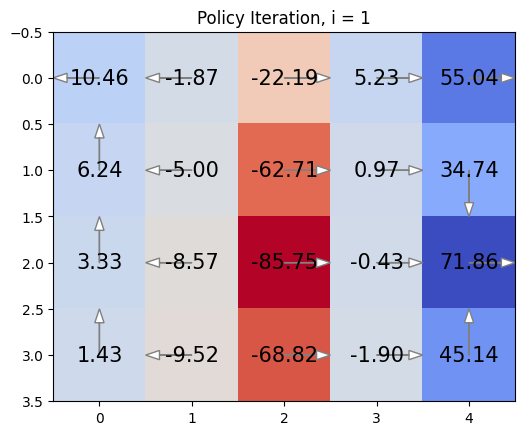
\includegraphics[width=.48\linewidth]{hw6/img_output/1c1.png}%
              }\hfill
              \subfloat[Iteration 2]{%
                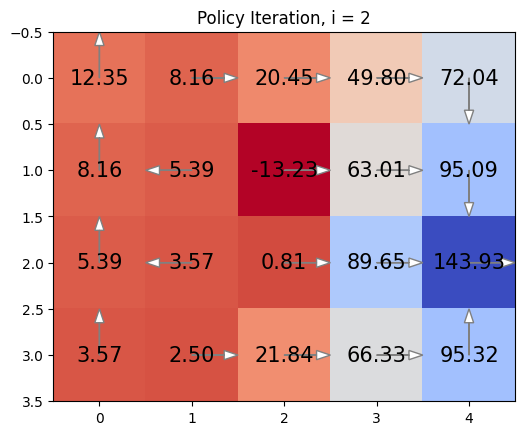
\includegraphics[width=.48\linewidth]{hw6/img_output/1c2.png}%
              }\\
              \subfloat[Iteration 3]{%
                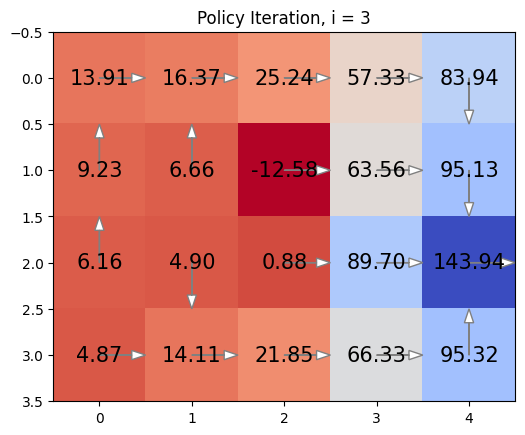
\includegraphics[width=.48\linewidth]{hw6/img_output/1c3.png}%
              }\hfill
              \subfloat[Iteration 4]{%
                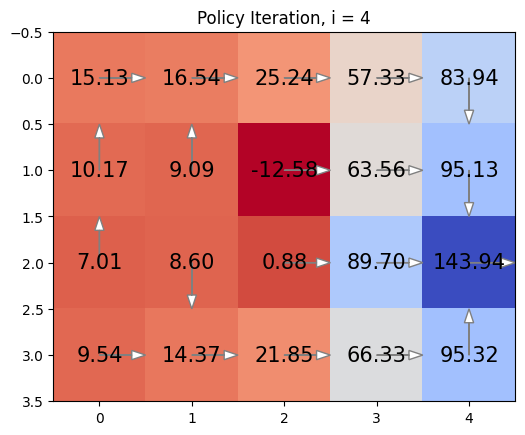
\includegraphics[width=.48\linewidth]{hw6/img_output/1c4.png}%
              }
            \end{figure}
            
            \newpage
            \item For all values of $ct$ (0.01, 0.001, 0.0001), it took 5 iterations to converge. Thus, changing $ct$ seems to have no affect on the number of iterations until convergence.
            \begin{figure}[htbp]
              \centering
              \subfloat[ct = 0.01]{%
                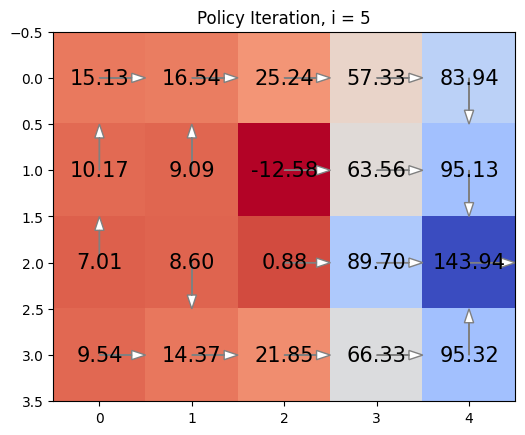
\includegraphics[width=.48\linewidth]{hw6/img_output/1dct0.01.png}%
              }\hfill
              \subfloat[ct = 0.001]{%
                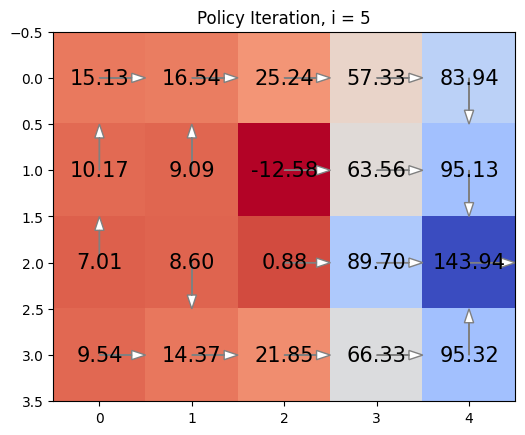
\includegraphics[width=.48\linewidth]{hw6/img_output/1dct0.001.png}%
              }\\
              \subfloat[ct = 0.0001 3]{%
                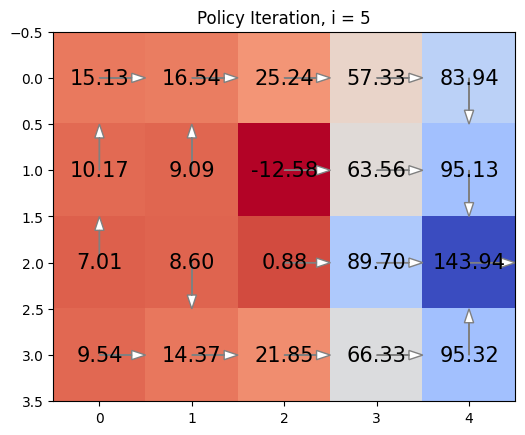
\includegraphics[width=.48\linewidth]{hw6/img_output/1dct0.0001.png}%
              }
            \end{figure}
        \end{enumerate}
        
        \item
        \begin{enumerate}
            \item Done. See code in supplemental materials.
            \newpage
            \item Done. 
            \begin{figure}[htbp]
              \centering
              \subfloat[Iteration 1]{%
                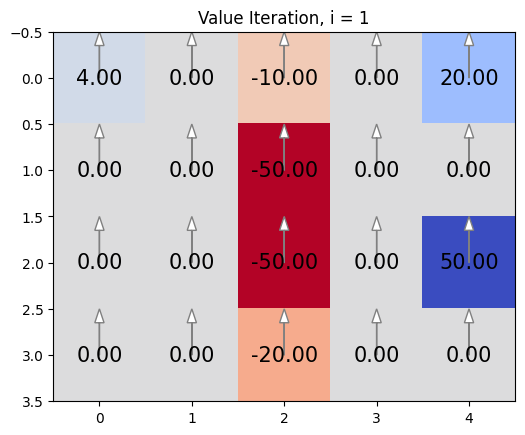
\includegraphics[width=.48\linewidth]{hw6/img_output/2b1.png}%
              }\hfill
              \subfloat[Iteration 2]{%
                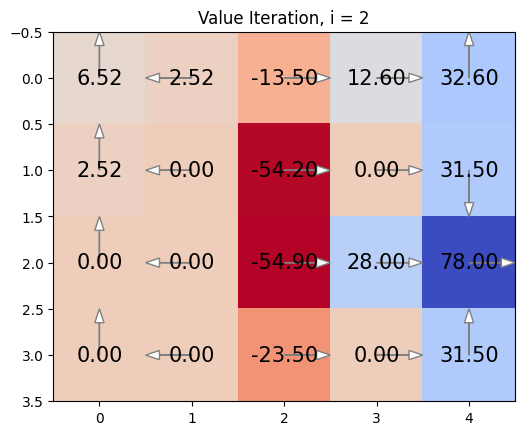
\includegraphics[width=.48\linewidth]{hw6/img_output/2b2.png}%
              }\\
              \subfloat[Iteration 3]{%
                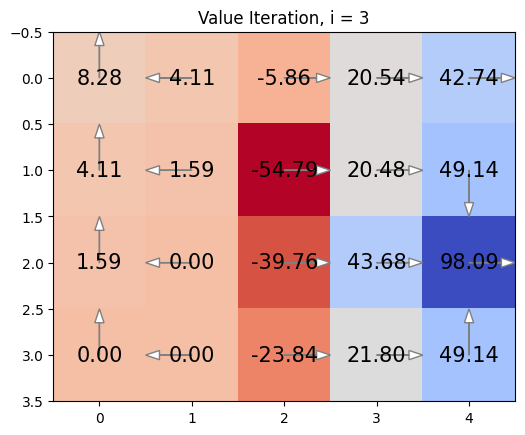
\includegraphics[width=.48\linewidth]{hw6/img_output/2b3.png}%
              }\hfill
              \subfloat[Iteration 4]{%
                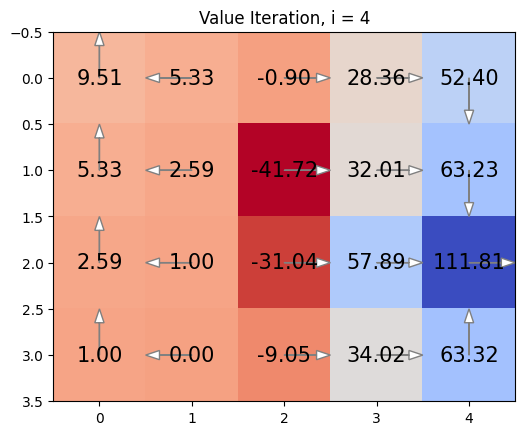
\includegraphics[width=.48\linewidth]{hw6/img_output/2b4.png}%
              }
            \end{figure}

            \newpage 
            \item When $ct = 0.01$, the number of iterations until convergence is 25. When $ct = 0.001$, the number of iterations until convergence is 31. When $ct = 0.0001$, the number of iterations until convergence is 38. Thus, we see a pattern of smaller $ct$ values leading to longer convergence times, which makes sense intuitively since tighter convergence tolerances impose a stricter stopping criterion on the maximum change and thus necessitate more iterations.
            \begin{figure}[htbp]
              \centering
              \subfloat[ct = 0.01]{%
                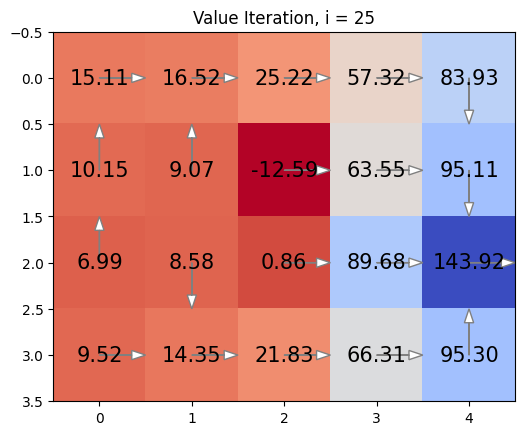
\includegraphics[width=.48\linewidth]{hw6/img_output/2cct0.01.png}%
              }\hfill
              \subfloat[ct = 0.001]{%
                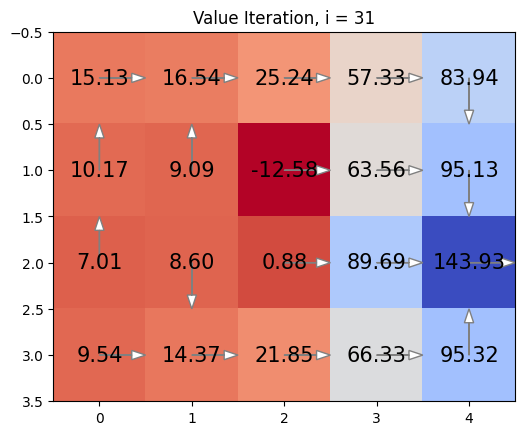
\includegraphics[width=.48\linewidth]{hw6/img_output/2cct0.001.png}%
              }\\
              \subfloat[ct = 0.0001 3]{%
                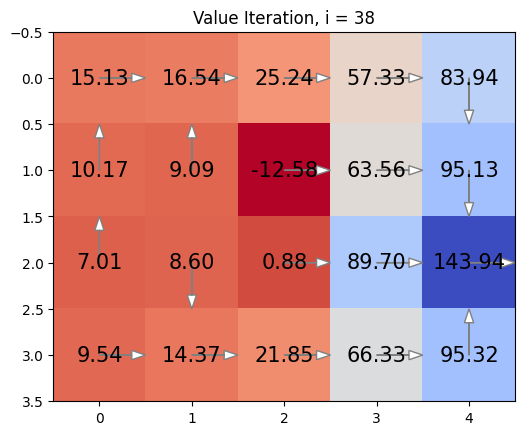
\includegraphics[width=.48\linewidth]{hw6/img_output/2cct0.0001.png}%
              }
            \end{figure}
        \end{enumerate}

        \item Policy iteration was faster than value iteration for every value of $ct$ that was tested. While value iteration took around 1.8-3 seconds to converge (for the values of $ct$ tested), policy iteration took 0.4 seconds every time, which makes sense since the convergence iteration was the same across all values of $ct$. Moreover, the number of iterations until convergence for policy iteration was lower across all values of $ct$ than value iteration. However, it seemed like policy iteration was slower per iteration compared to value iteration.

        \item When $\gamma=0.6$ the learned policy is very short sighted: the agent always moves toward the nearest reward of 4 and ignores the distant 20 and 50 point goal. As $\gamma$ increases to 0.7 and 0.8, the policy gradually shifts agents will bypass small gains and navigate around penalties to reach the 20 point or 50 point cells. By $\gamma=0.9$ the policy points almost uniformly toward the 50‐point target, even if it lies farther away and requires passing through negative states. This behavior is because increasing $\gamma$ places more weight on distant rewards which incentivizes the agent to prioritize heading towards the 50 state. Thus higher $\gamma$ yields more farsighted behavior. Increasing $\gamma$ did not seem to have a significant effect on runtime, with only a marginal increase in runtime due to more iterations for convergence.
        \begin{figure}[htbp]
              \centering
              \subfloat[ $\gamma$ = 0.6]{%
                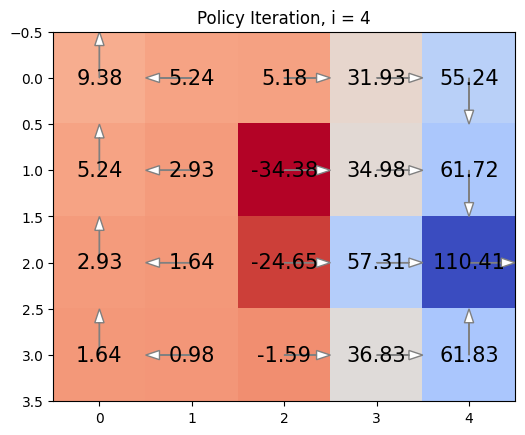
\includegraphics[width=.48\linewidth]{hw6/img_output/2.40.6.png}%
              }\hfill
              \subfloat[$\gamma$ = 0.7]{%
                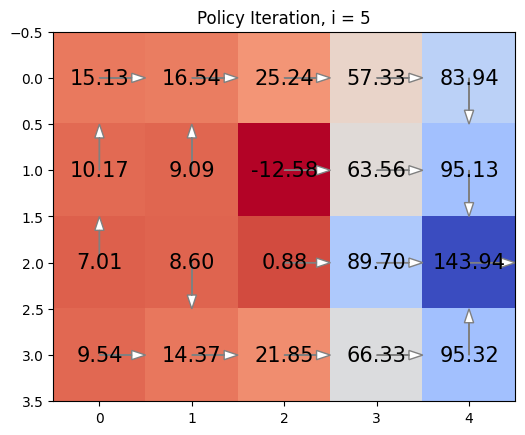
\includegraphics[width=.48\linewidth]{hw6/img_output/2.40.7.png}%
              }\\
              \subfloat[$\gamma$ = 0.8]{%
                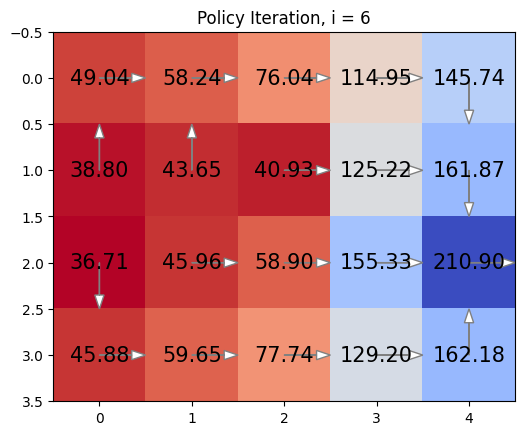
\includegraphics[width=.48\linewidth]{hw6/img_output/2.40.8.png}%
              }\hfill
              \subfloat[$\gamma$ = 0.9]{%
                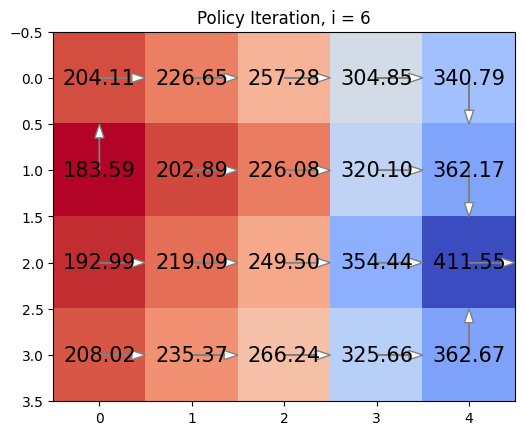
\includegraphics[width=.48\linewidth]{hw6/img_output/2.40.9.png}%
              }
            \end{figure}

        \item  When $\gamma$ is very small, the agent cares almost only about the immediate next step, so it will go to the nearest reward and stop. This would result in the agent navigating to the 4 state and then stopping after. As $\gamma$ increases, the agent begins to value future gains more and will accept a longer path if it leads to a larger payoff. At intermediate values of $\gamma$ it may skip a small nearby reward in favor of a medium one that lies a bit farther away  (which is why at $\gamma = 0.7$ in part (4) the agent continues past the 20 state). When $\gamma$ is close to one, the agent plans to maximize its total haul and would head directly for the largest prize regardless of distance. Thus the optimal policy gradually shifts from purely greedy local moves toward long term planning as $\gamma$ grows.

        \item By using the approach we took (modeling the problem), we avoid doing trial and error on the real machine which as several advantages. The upside is that, using RL on the actual robot is logistically time consuming since the robot would take time to travel to different locations or could run out of battery which then would require time to charge. Thus, simulating the environment as Gridworld using code significantly speeds up the rate at which you could solve the original task. Moreover, we don't risk wearing the sensitive parts of the floor or wearing down our robot while learning optimal policy. The downside is that we must trust the model: if the actual transitions or rewards differ, the policy may fail or not apply to the actual real world task.

        \item We see that when $\gamma = 0.7$ the resulting policy accomplishes what we would like our robot to do, hitting both the intermediary rewards (corresponding to the two parts) and ending at the goal location. However, the other policies learned do not accomplish the original task completely. We made three simplifying modeling choices that detract from solving the real world task. First, the state is just the robots location and contains no record of which parts have been picked up. Second, reaching a part cell immediately ends the trial with a one time reward, instead of requiring the agent to pick up the part and then continue to the goal (it doesn't matter that the agent reaches the part, it matters that the part is delivered to the goal). Third, we discretized the workspace into uniform cells, ignoring that in a real robot setting the cost or reward can vary continuously (for example, damage risk rises near delicate floor areas and can’t be captured by a single cell value). 
        \\
        \\
        Each of these choices inhibits the policy from completing pickup and delivery. Without inventory flags the agent cannot plan to pickup both the parts. By absorbing rewards at first pickup, the agent has no further incentive to deliver the part to the goal. Finally, with coarse uniform cells the agent does not have the granularity to find the most optimal policy and instead must contend with jumping between these discrete cells. In order to better represent and achieve the real objective, we would need to track the inventory of the agent and alter the reward of each state depending on this inventory. Moreover, we would need to increase the granularity of the state space to better reflect risks and rewards.
        
        


    \end{enumerate}
=======
	Your solution here.
>>>>>>> 029a483aa01e3c3745c42e8094d4dbc952e22f1f
\end{solution}


\begin{problem}[Reinforcement Learning, 20 pts]
  In 2013, the mobile game \emph{Flappy Bird} took the world by storm. You'll be developing a Q-learning agent to play a similar game, \emph{Swingy Monkey} (See Figure~\ref{fig:swingy}).  In this game, you control a monkey that is trying to swing on vines and avoid tree trunks.  You can either make him jump to a new vine, or have him swing down on the vine he's currently holding.  You get points for successfully passing tree trunks without hitting them, falling off the bottom of the screen, or jumping off the top.  There are some sources of randomness: the monkey's jumps are sometimes higher than others, the gaps in the trees vary vertically, the gravity varies from game to game, and the distances between the trees are different.  You can play the game directly by pushing a key on the keyboard to make the monkey jump.  However, your objective is to build an agent that \emph{learns} to play on its own. 
  
   You will need to install the \verb|pygame| module
  (\url{http://www.pygame.org/wiki/GettingStarted}).
  

\textbf{Task:}
Your task is to use Q-learning to find a policy for the monkey that can navigate the trees.  The \verb|homework6_soln.ipynb| file contains starter code for setting up your learner that interacts with the game. This is the \textbf{only code file} you need to modify. At the beginning of the code, you will import the \verb|SwingyMonkey| class, which is the implementation of the game that has already been completed for you. Note that by default we have you import this class from the file \verb|SwingyMonkeyNoAnimation.py|, which allows you to speed up testing. To actually see the game animation, you can instead import from \verb|SwingyMonkey.py|. Additionally, we provide a video of the staff Q-Learner playing the game at \url{https://youtu.be/xRD6xBQbauw}.  It figures out a reasonable policy in a few iterations.
You'll be responsible for implementing the Python function  \verb|action_callback|. The action callback will take in a dictionary that describes the current state of the game and return an action for the next time step.  This will be a binary action, where 0 means to swing downward and 1 means to jump up.  The dictionary you get for the state looks like this:
\begin{csv}
{ 'score': <current score>,
  'tree': { 'dist': <pixels to next tree trunk>,
            'top':  <height of top of tree trunk gap>,
            'bot':  <height of bottom of tree trunk gap> },
  'monkey': { 'vel': <current monkey y-axis speed>,
              'top': <height of top of monkey>,
              'bot': <height of bottom of monkey> }}
\end{csv}
All of the units here (except score) will be in screen pixels. Figure~\ref{fig:swingy-ann} shows these graphically. 
Note that since the state space is very large (effectively continuous), the monkey's relative position needs to be discretized into bins. The pre-defined function \verb|discretize_state| does this for you.

\textbf{Requirements}
\\
\textit{Code}: First, you should implement Q-learning with an
$\epsilon$-greedy policy yourself. You can increase the performance by
trying out different parameters for the learning rate $\alpha$,
discount rate $\gamma$, and exploration rate $\epsilon$. \emph{Do not use outside RL code for this assignment.} Second, you should use a method of your choice to further improve the performance. This could be inferring gravity at each epoch (the gravity varies from game to game), updating the reward function, trying decaying epsilon greedy functions, changing the features in the state space, and more. One of our staff solutions got scores over 800 before the 100th epoch, but you are only expected to reach scores over 50 at least once before the 100th epoch. {\bf Make sure to turn in your code!} \\\\

\textit{Evaluation}: In 1-2 paragraphs, explain how your agent performed and what decisions you made and why. Make sure to provide evidence where necessary to explain your decisions. You must include in your write up at least one plot or table that details the performances of parameters tried (i.e. plots of score vs. epoch number for different parameters). \\\\

\textit{Note}: Note that you can simply discretize the state and action spaces and run the Q-learning algorithm. There is no need to use complex models such as neural networks to solve this problem, but you may do so as a fun exercise.

\end{problem}
<<<<<<< HEAD

=======
>>>>>>> 029a483aa01e3c3745c42e8094d4dbc952e22f1f
\begin{figure}[H]
    \centering%
    \subfloat[SwingyMonkey Screenshot]{%
        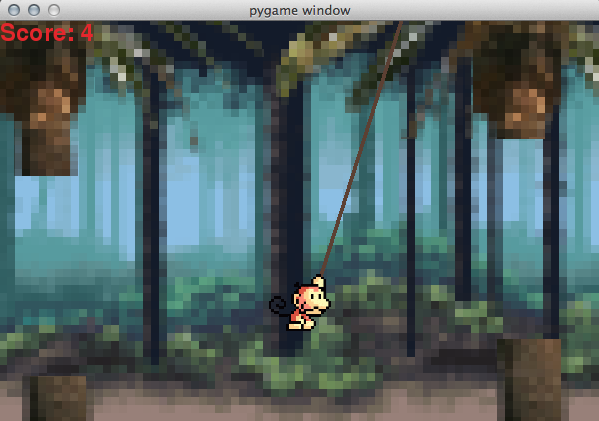
\includegraphics[width=0.48\textwidth]{img_input/swingy}
        \label{fig:swingy}
    }\hfill
    \subfloat[SwingyMonkey State]{%
        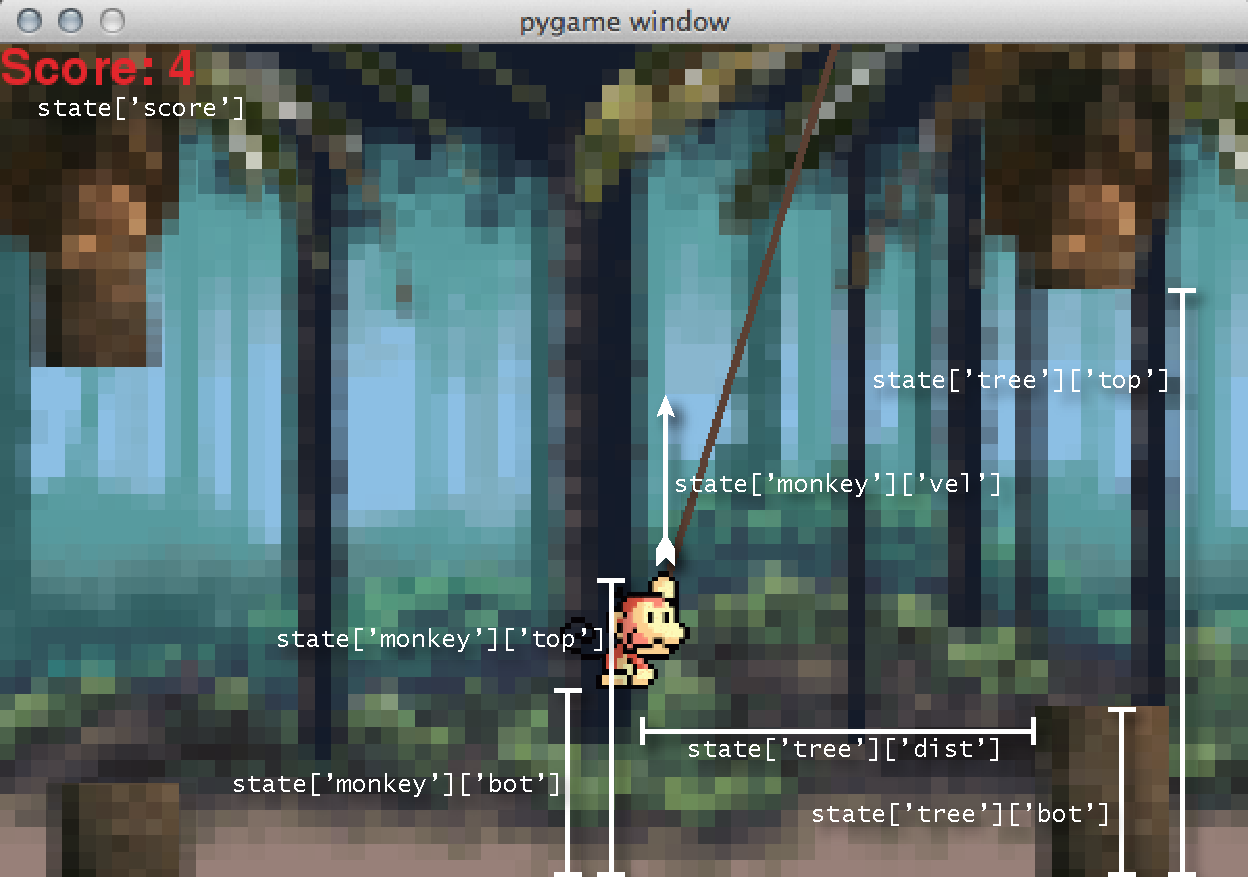
\includegraphics[width=0.48\textwidth]{img_input/swingy-ann}
        \label{fig:swingy-ann}
    }
    \caption{(a) Screenshot of the Swingy Monkey game.  (b) Interpretations of various pieces of the state dictionary.}
<<<<<<< HEAD
\end{figure} 

\begin{solution}
Here are baseline results
\begin{figure}[H]
    \centering
    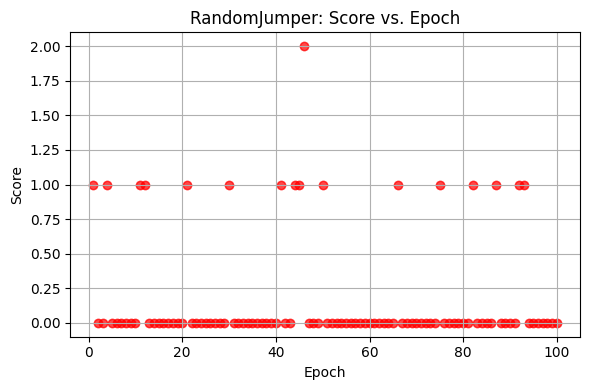
\includegraphics[width=0.5\linewidth]{hw6/img_output/baseline_random.png}
\end{figure}
\begin{figure}[H]
    \centering
    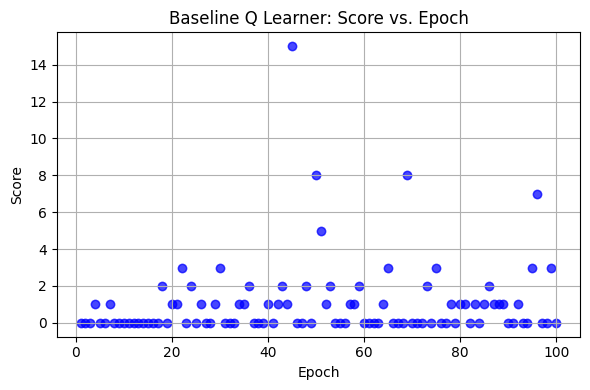
\includegraphics[width=0.5\linewidth]{hw6/img_output/baselineqlearn.png}
\end{figure}

On the basic Q learner, I tested 1000 hyperparameter combinations of $\alpha$, $\gamma$, and $\epsilon$ over five trials each and recorded mean, median, and max scores. The table below lists the top ten settings by mean score; the best configuration ($\alpha = 0.17$, $\gamma = 0.99$, $\epsilon = 0.0001$) achieved an average score of 70 and a peak of over 900. To better visualize learning dynamics, we picked the four highest mean hyperparameter settings and plotted score versus epoch in a $2 \times 2$ grid. In every case the agent scored near zero for the first 40 to 50 games, then suddenly discovered better strategies and began producing sporadic high score episodes. These results suggest that a high discount factor, moderate learning rate, and very low exploration strike the best balance between planning long term and finding a stable policy, so I carried these insights forward into our epsilon decay  learner.
\begin{table}[htbp]
\centering
\begin{tabular}{rrrrrr}
\hline
$\alpha$ & $\gamma$ & $\epsilon$ & mean score & median score & max score \\
\hline
0.167333 & 0.99 & 0.0001 & 70.170 & 1.8 & 906.2 \\
0.333667 & 0.99 & 0.0001 & 61.810 & 1.6 & 961.0 \\
0.278222 & 0.99 & 0.0001 & 59.446 & 1.4 & 658.6 \\
0.222778 & 0.88 & 0.0001 & 58.626 & 1.0 & 734.8 \\
0.056444 & 0.88 & 0.0001 & 55.394 & 1.5 & 740.6 \\
0.111889 & 0.55 & 0.0001 & 55.092 & 1.2 & 1063.0 \\
0.222778 & 0.99 & 0.0001 & 54.660 & 1.0 & 1170.4 \\
0.278222 & 0.77 & 0.0001 & 53.392 & 1.4 & 637.6 \\
0.278222 & 0.88 & 0.0001 & 52.548 & 1.6 & 781.4 \\
0.111889 & 0.99 & 0.0001 & 52.012 & 1.6 & 862.0 \\
\hline
\end{tabular}
\caption{Hyperparameter tuning results for the Q learner}

\end{table}
\begin{figure}
    \centering
    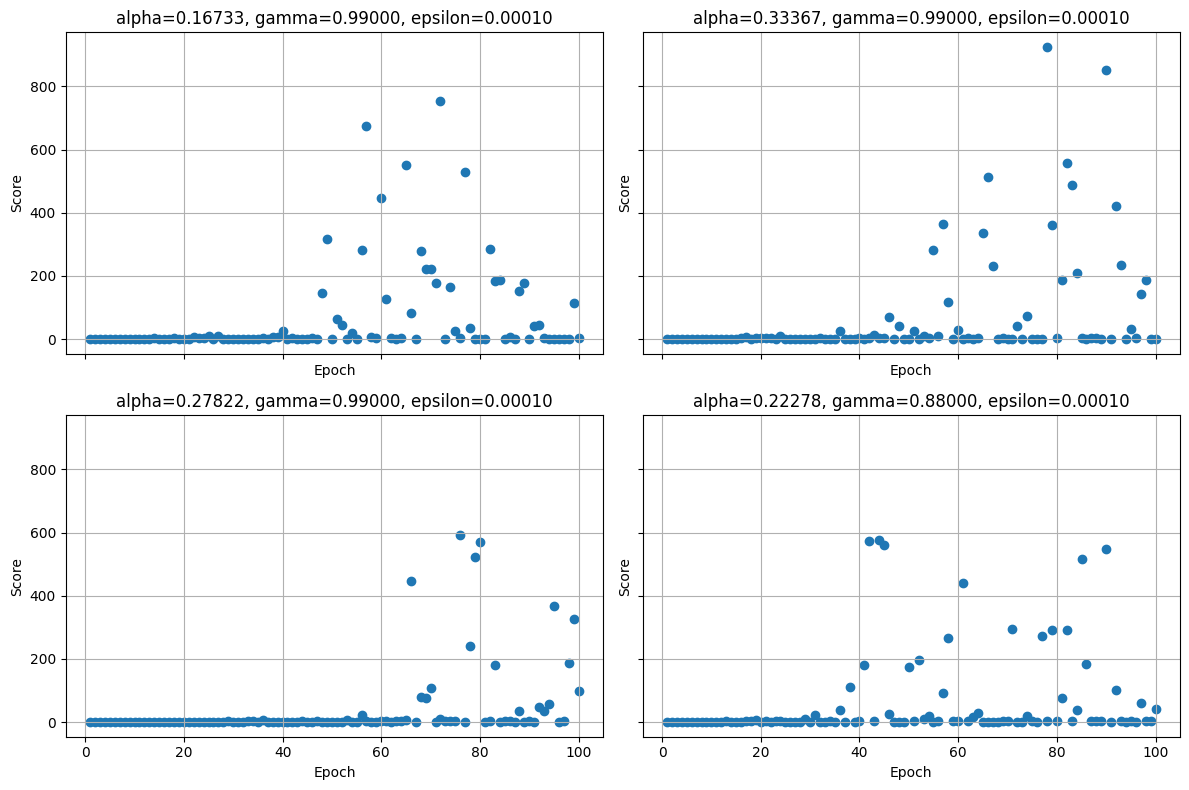
\includegraphics[width=0.8\linewidth]{hw6/img_output/p3plot1.png}
    \caption{Best 4 Hyperparameter Settings on Default Q Learner}
\end{figure}

Next, I implemented Q learning with an epsilon greedy policy by modifying the Q-learner code and then tested a linear decay schedule where epsilon is multiplied by a fixed decay factor each episode down to a small floor.  The table above shows that the best linear decay setting achieves a mean score of about 68, which is slightly below our tuned static epsilon high‐gamma result (mean around 70) but far above the untuned baseline and random jumper. I think this is because linear decay reduces $\epsilon$ by the same fraction each episode, so it never adapts to how quickly the agent is actually learning. Early on this means the exploration rate stays too high for too long, washing out emerging Q value patterns and slowing down the discovery of good trajectories. Later in training $\epsilon$ remains above the ideal exploitation threshold, preventing the agent from consistently following the best moves it has already learned. Because a fixed decay schedule ignores the agent’s real time performance, exploration and exploitation stay out of balance (too much randomness when we should exploit learned value patterns and insufficient exploration when we need to try new paths) so average scores plateau rather than improve. Thus, I believe a decay rule that responds to performance (ie. stepping down only after steady improvement) would align exploration with the agent’s needs and boost final results. Despite this, mean scores of 68 versus baseline near zero confirm that even a simple decay rule helps, and tuning the decay rate or lowering the minimum epsilon further should close the remaining gap. I also tried an exponential decay schedule, but it only matched the baseline Q learners performance. In this case, I believe epsilon either dropped too quickly at the start, cutting off needed exploration, or leveled off too slowly above the optimal floor, so the agent never settled on a stable policy.

\begin{table}[htbp]
\centering
\begin{tabular}{rrrrrrrr}
\hline
$\alpha$ & $\gamma$ & $\epsilon$ & $\epsilon_{decay}$ & $\min_{\epsilon}$ & mean score & median score & max score \\
\hline
0.100000 & 0.893333 & 0.100000 & 0.90 & 0.0001 & 67.632 & 1.7 & 826.6 \\
0.233333 & 0.990000 & 0.100000 & 0.90 & 0.0001 & 54.408 & 1.3 & 782.0 \\
0.100000 & 0.893333 & 0.500000 & 0.90 & 0.0001 & 53.814 & 1.0 & 899.6 \\
0.100000 & 0.893333 & 0.100000 & 0.93 & 0.0001 & 50.242 & 1.1 & 701.0 \\
0.100000 & 0.990000 & 0.100000 & 0.90 & 0.0001 & 49.240 & 1.2 & 941.4 \\
0.233333 & 0.893333 & 0.100000 & 0.90 & 0.0001 & 47.672 & 1.0 & 646.8 \\
0.100000 & 0.893333 & 0.366667 & 0.90 & 0.0001 & 45.078 & 1.0 & 809.4 \\
0.233333 & 0.893333 & 0.233333 & 0.90 & 0.0001 & 42.542 & 1.0 & 731.6 \\
0.233333 & 0.990000 & 0.100000 & 0.93 & 0.0001 & 42.240 & 1.0 & 840.0 \\
0.100000 & 0.796667 & 0.233333 & 0.90 & 0.0001 & 41.736 & 1.0 & 725.4 \\
\hline
\end{tabular}
\caption{Hyperparameter tuning results for the linear‐decay Q‐learner}
\end{table}
\end{solution}

\begin{lstlisting}
class RandomJumper(object):
    """
    This agent jumps randomly.
    """

    def __init__(self):
        self.last_state = None
        self.last_action = None
        self.last_reward = None

        # We initialize our Q-value grid that has an entry for each action and state.
        # (action, rel_x, rel_y)
        self.Q = np.zeros((2, X_SCREEN // X_BINSIZE, Y_SCREEN // Y_BINSIZE))

    def reset(self):
        self.last_state = None
        self.last_action = None
        self.last_reward = None

    def discretize_state(self, state):
        """
        Discretize the position space to produce binned features.
        rel_x = the binned relative horizontal distance between the monkey and the tree
        rel_y = the binned relative vertical distance between the monkey and the tree
        """

        rel_x = int((state["tree"]["dist"]) // X_BINSIZE)
        rel_y = int((state["tree"]["top"] - state["monkey"]["top"]) // Y_BINSIZE)
        return (rel_x, rel_y)

    def action_callback(self, state):
        """
        Implement this function to learn things and take actions.
        Return 0 if you don't want to jump and 1 if you do.
        """

        new_action = npr.rand() < 0.1
        new_state = state

        self.last_action = new_action
        self.last_state = new_state

        return self.last_action

    def reward_callback(self, reward):
        """This gets called so you can see what reward you get."""

        self.last_reward = reward

import random
import numpy as np

class Learner(object):
    '''
    This agent uses Q-learning!
    '''

    def __init__(self, alpha=0.1, gamma=0.9, epsilon=0.1):
        self.alpha = alpha
        self.gamma = gamma
        self.epsilon = epsilon

        self.Q = np.zeros((2, X_SCREEN  // X_BINSIZE, Y_SCREEN  // Y_BINSIZE))

        self.last_state = None
        self.last_action = None
        self.last_reward = 0
        
    def discretize_state(self, state):
        """
        Discretize the position space to produce binned features.
        rel_x = the binned relative horizontal distance between the monkey and the tree
        rel_y = the binned relative vertical distance between the monkey and the tree
        """
        rel_x = int((state["tree"]["dist"]) // X_BINSIZE)
        rel_y = int((state["tree"]["top"] - state["monkey"]["top"]) // Y_BINSIZE)
        return (rel_x, rel_y)
    
    def reset(self):
        self.last_state = None
        self.last_action = None
        self.last_reward = None

    def action_callback(self, state):
        '''
        Implement this function to learn things and take actions.
        Return 0 if you don't want to jump and 1 if you do.
        '''
        s = self.discretize_state(state)

        if self.last_state is not None:
            lx, ly = self.last_state
            old_q = self.Q[self.last_action, lx, ly]
            future_value = np.max(self.Q[:, s[0], s[1]])
            self.Q[self.last_action, lx, ly] = (old_q + self.alpha* (self.last_reward + self.gamma * future_value - old_q))

        if random.random() < self.epsilon:
            a = random.randint(0, 1)
        else:
            qvals = self.Q[:, s[0], s[1]]
            a = int(np.random.choice(np.flatnonzero(qvals == qvals.max())))

        self.last_state = s
        self.last_action = a

        return a
    
    def reward_callback(self, reward):
        '''This gets called so you can see what reward you get.'''
        self.last_reward = reward

import matplotlib.pyplot as plt

random_hist = []
agent_random = RandomJumper()
run_games(agent_random, random_hist, iters=100, t_len=100)

plt.figure(figsize=(6,4))
epochs = np.arange(1, len(random_hist)+1)
plt.scatter(epochs, random_hist, color='red', alpha=0.6)
plt.scatter(epochs, random_hist, color='red', alpha=0.3)
plt.title('RandomJumper: Score vs. Epoch')
plt.xlabel('Epoch')
plt.ylabel('Score')
plt.grid(True)
plt.tight_layout()
plt.show()

baseline_hist = []
agent_baseline = Learner()
run_games(agent_baseline, baseline_hist, iters=100, t_len=100)

plt.figure(figsize=(6,4))
epochs = np.arange(1, len(baseline_hist)+1)
plt.scatter(epochs, baseline_hist, color='blue', alpha=0.6)
plt.scatter(epochs, baseline_hist, color='blue', alpha=0.3)
plt.title('Baseline Q Learner: Score vs. Epoch')
plt.xlabel('Epoch')
plt.ylabel('Score')
plt.grid(True)
plt.tight_layout()
plt.show()

import itertools
import pandas as pd
import numpy as np

param_grid = {
    'alpha': np.linspace(0.001, 0.5, 10),
    'gamma': np.linspace(0, 0.99, 10),
    'epsilon': np.linspace(0.0001, 0.3, 10) 
}

n_trials = 5
results = []

for alpha, gamma, epsilon in itertools.product(
        param_grid['alpha'],
        param_grid['gamma'],
        param_grid['epsilon']
    ):
    mean_scores   = []
    median_scores = []
    max_scores    = []
    
    for _ in range(n_trials):
        learner = Learner(alpha=alpha, gamma=gamma, epsilon=epsilon)
        hist = []
        run_games(learner, hist, iters=100, t_len=5)
        
        mean_scores.append(np.mean(hist))
        median_scores.append(np.median(hist))
        max_scores.append(np.max(hist))
    
    results.append({
        'alpha': alpha,
        'gamma': gamma,
        'epsilon': epsilon,
        'mean_score':   np.mean(mean_scores),
        'median_score': np.mean(median_scores),
        'max_score':    np.mean(max_scores)
    })

df = pd.DataFrame(results)
print(df.sort_values('mean_score', ascending=False).head(10))
print(df.sort_values('max_score', ascending=False).head(10))

import matplotlib.pyplot as plt

top4 = df.sort_values('max_score', ascending=False).head(4)

fig, axes = plt.subplots(2, 2, figsize=(12, 8), sharex=True, sharey=True)

axes = axes.flatten()

for ax, (_, row) in zip(axes, top4.iterrows()):
    alpha = row['alpha']
    gamma = row['gamma']
    epsilon = row['epsilon']
    learner = Learner(alpha=alpha, gamma=gamma, epsilon=epsilon)
    hist = []
    run_games(learner, hist, iters=100, t_len=25)
    epochs = np.arange(1, len(hist) + 1)
    
    ax.scatter(epochs, hist)
    ax.set_title(f'alpha={alpha:.5f}, gamma={gamma:.5f}, epsilon={epsilon:.5f}')
    ax.set_xlabel('Epoch')
    ax.set_ylabel('Score')
    ax.grid(True)

plt.tight_layout()
plt.show()

import random
import numpy as np

class LearnerDecay(object):
    '''
    This agent uses Q-learning (with epsilon decay)!
    '''

    def __init__(self, alpha=0.1, gamma=0.9, epsilon=0.5, epsilon_decay=0.95, min_epsilon=0.01):
        self.alpha = alpha
        self.gamma = gamma
        self.epsilon = epsilon

        self.epsilon_decay = epsilon_decay
        self.min_epsilon   = min_epsilon
        self.episode       = 0

        self.Q = np.zeros((2,X_SCREEN  // X_BINSIZE, Y_SCREEN  // Y_BINSIZE))

        self.last_state  = None
        self.last_action = None
        self.last_reward = 0
        
    def discretize_state(self, state):
        """
        Discretize the position space to produce binned features.
        rel_x = the binned relative horizontal distance between the monkey and the tree
        rel_y = the binned relative vertical distance between the monkey and the tree
        """
        rel_x = int((state["tree"]["dist"]) // X_BINSIZE)
        rel_y = int((state["tree"]["top"] - state["monkey"]["top"]) // Y_BINSIZE)
        return (rel_x, rel_y)
    
    def reset(self):
        self.last_state = None
        self.last_action = None
        self.last_reward = None
        
        self.episode += 1
        self.epsilon = max(self.min_epsilon, self.epsilon * self.epsilon_decay)

    def action_callback(self, state):
        '''
        Implement this function to learn things and take actions.
        Return 0 if you don't want to jump and 1 if you do.
        '''
        s = self.discretize_state(state)

        if self.last_state is not None:
            lx, ly = self.last_state
            old_q = self.Q[self.last_action, lx, ly]
            future_value = np.max(self.Q[:, s[0], s[1]])
            self.Q[self.last_action, lx, ly] = (old_q + self.alpha * (self.last_reward+ self.gamma * future_value- old_q))

        if random.random() < self.epsilon:
            a = random.randint(0, 1)
        else:
            qvals = self.Q[:, s[0], s[1]]
            a = int(np.random.choice(np.flatnonzero(qvals == qvals.max())))

        self.last_state  = s
        self.last_action = a

        return a
    
    def reward_callback(self, reward):
        '''This gets called so you can see what reward you get.'''
        self.last_reward = reward

import itertools
import pandas as pd

param_grid = {
    'alpha':         np.linspace(0.1, 0.5, 4),
    'gamma':         np.linspace(0.7, 0.99, 4),
    'epsilon':       np.linspace(0.1, 0.5, 4),
    'epsilon_decay': np.linspace(0.90, 0.99, 4),
    'min_epsilon':   np.linspace(0.0001, 0.01, 4)
}

n_trials = 5
results = []

for alpha, gamma, epsilon, epsilon_decay, min_epsilon in itertools.product(
        param_grid['alpha'],
        param_grid['gamma'],
        param_grid['epsilon'],
        param_grid['epsilon_decay'],
        param_grid['min_epsilon']
    ):
    mean_scores   = []
    median_scores = []
    max_scores    = []
    
    for _ in range(n_trials):
        learner = LearnerDecay(
            alpha=alpha,
            gamma=gamma,
            epsilon=epsilon,
            epsilon_decay=epsilon_decay,
            min_epsilon=min_epsilon
        )
        hist = []
        run_games(learner, hist, iters=100, t_len=5)
        
        mean_scores.append(np.mean(hist))
        median_scores.append(np.median(hist))
        max_scores.append(np.max(hist))
    
    results.append({
        'alpha':         alpha,
        'gamma':         gamma,
        'epsilon':       epsilon,
        'epsilon_decay': epsilon_decay,
        'min_epsilon':   min_epsilon,
        'mean_score':    np.mean(mean_scores),
        'median_score':  np.mean(median_scores),
        'max_score':     np.mean(max_scores)
    })

df_decay = pd.DataFrame(results)
print(df_decay.sort_values('mean_score', ascending=False).head(10))

\end{lstlisting}
=======
\end{figure}
    

\begin{solution}
	Your solution here.
\end{solution}

>>>>>>> 029a483aa01e3c3745c42e8094d4dbc952e22f1f
\newpage
%%%%%%%%%%%%%%%%%%%%%%%%%%%%%%%%%%%%%%%%%%%%%
% Name and Calibration
%%%%%%%%%%%%%%%%%%%%%%%%%%%%%%%%%%%%%%%%%%%%%
\newpage
\subsection*{Name}
<<<<<<< HEAD
Jaray Liu
\subsection*{Collaborators and Resources}
Whom did you work with, and did you use any resources beyond cs181-textbook and your notes?
I searched online for good non linear decay functions and found this wiki article that was very helpful:
\url{https://en.wikipedia.org/wiki/Exponential_decay}
=======
\subsection*{Collaborators and Resources}
Whom did you work with, and did you use any resources beyond cs181-textbook and your notes?
>>>>>>> 029a483aa01e3c3745c42e8094d4dbc952e22f1f

\end{document}
